% Options for packages loaded elsewhere
% Options for packages loaded elsewhere
\PassOptionsToPackage{unicode}{hyperref}
\PassOptionsToPackage{hyphens}{url}
\PassOptionsToPackage{dvipsnames,svgnames,x11names}{xcolor}
%
\documentclass[
  letterpaper,
  DIV=11,
  numbers=noendperiod,
  oneside]{scrartcl}
\usepackage{xcolor}
\usepackage[left=1in,marginparwidth=2.0666666666667in,textwidth=4.1333333333333in,marginparsep=0.3in]{geometry}
\usepackage{amsmath,amssymb}
\setcounter{secnumdepth}{5}
\usepackage{iftex}
\ifPDFTeX
  \usepackage[T1]{fontenc}
  \usepackage[utf8]{inputenc}
  \usepackage{textcomp} % provide euro and other symbols
\else % if luatex or xetex
  \usepackage{unicode-math} % this also loads fontspec
  \defaultfontfeatures{Scale=MatchLowercase}
  \defaultfontfeatures[\rmfamily]{Ligatures=TeX,Scale=1}
\fi
\usepackage{lmodern}
\ifPDFTeX\else
  % xetex/luatex font selection
\fi
% Use upquote if available, for straight quotes in verbatim environments
\IfFileExists{upquote.sty}{\usepackage{upquote}}{}
\IfFileExists{microtype.sty}{% use microtype if available
  \usepackage[]{microtype}
  \UseMicrotypeSet[protrusion]{basicmath} % disable protrusion for tt fonts
}{}
\makeatletter
\@ifundefined{KOMAClassName}{% if non-KOMA class
  \IfFileExists{parskip.sty}{%
    \usepackage{parskip}
  }{% else
    \setlength{\parindent}{0pt}
    \setlength{\parskip}{6pt plus 2pt minus 1pt}}
}{% if KOMA class
  \KOMAoptions{parskip=half}}
\makeatother
% Make \paragraph and \subparagraph free-standing
\makeatletter
\ifx\paragraph\undefined\else
  \let\oldparagraph\paragraph
  \renewcommand{\paragraph}{
    \@ifstar
      \xxxParagraphStar
      \xxxParagraphNoStar
  }
  \newcommand{\xxxParagraphStar}[1]{\oldparagraph*{#1}\mbox{}}
  \newcommand{\xxxParagraphNoStar}[1]{\oldparagraph{#1}\mbox{}}
\fi
\ifx\subparagraph\undefined\else
  \let\oldsubparagraph\subparagraph
  \renewcommand{\subparagraph}{
    \@ifstar
      \xxxSubParagraphStar
      \xxxSubParagraphNoStar
  }
  \newcommand{\xxxSubParagraphStar}[1]{\oldsubparagraph*{#1}\mbox{}}
  \newcommand{\xxxSubParagraphNoStar}[1]{\oldsubparagraph{#1}\mbox{}}
\fi
\makeatother

\usepackage{color}
\usepackage{fancyvrb}
\newcommand{\VerbBar}{|}
\newcommand{\VERB}{\Verb[commandchars=\\\{\}]}
\DefineVerbatimEnvironment{Highlighting}{Verbatim}{commandchars=\\\{\}}
% Add ',fontsize=\small' for more characters per line
\usepackage{framed}
\definecolor{shadecolor}{RGB}{241,243,245}
\newenvironment{Shaded}{\begin{snugshade}}{\end{snugshade}}
\newcommand{\AlertTok}[1]{\textcolor[rgb]{0.68,0.00,0.00}{#1}}
\newcommand{\AnnotationTok}[1]{\textcolor[rgb]{0.37,0.37,0.37}{#1}}
\newcommand{\AttributeTok}[1]{\textcolor[rgb]{0.40,0.45,0.13}{#1}}
\newcommand{\BaseNTok}[1]{\textcolor[rgb]{0.68,0.00,0.00}{#1}}
\newcommand{\BuiltInTok}[1]{\textcolor[rgb]{0.00,0.23,0.31}{#1}}
\newcommand{\CharTok}[1]{\textcolor[rgb]{0.13,0.47,0.30}{#1}}
\newcommand{\CommentTok}[1]{\textcolor[rgb]{0.37,0.37,0.37}{#1}}
\newcommand{\CommentVarTok}[1]{\textcolor[rgb]{0.37,0.37,0.37}{\textit{#1}}}
\newcommand{\ConstantTok}[1]{\textcolor[rgb]{0.56,0.35,0.01}{#1}}
\newcommand{\ControlFlowTok}[1]{\textcolor[rgb]{0.00,0.23,0.31}{\textbf{#1}}}
\newcommand{\DataTypeTok}[1]{\textcolor[rgb]{0.68,0.00,0.00}{#1}}
\newcommand{\DecValTok}[1]{\textcolor[rgb]{0.68,0.00,0.00}{#1}}
\newcommand{\DocumentationTok}[1]{\textcolor[rgb]{0.37,0.37,0.37}{\textit{#1}}}
\newcommand{\ErrorTok}[1]{\textcolor[rgb]{0.68,0.00,0.00}{#1}}
\newcommand{\ExtensionTok}[1]{\textcolor[rgb]{0.00,0.23,0.31}{#1}}
\newcommand{\FloatTok}[1]{\textcolor[rgb]{0.68,0.00,0.00}{#1}}
\newcommand{\FunctionTok}[1]{\textcolor[rgb]{0.28,0.35,0.67}{#1}}
\newcommand{\ImportTok}[1]{\textcolor[rgb]{0.00,0.46,0.62}{#1}}
\newcommand{\InformationTok}[1]{\textcolor[rgb]{0.37,0.37,0.37}{#1}}
\newcommand{\KeywordTok}[1]{\textcolor[rgb]{0.00,0.23,0.31}{\textbf{#1}}}
\newcommand{\NormalTok}[1]{\textcolor[rgb]{0.00,0.23,0.31}{#1}}
\newcommand{\OperatorTok}[1]{\textcolor[rgb]{0.37,0.37,0.37}{#1}}
\newcommand{\OtherTok}[1]{\textcolor[rgb]{0.00,0.23,0.31}{#1}}
\newcommand{\PreprocessorTok}[1]{\textcolor[rgb]{0.68,0.00,0.00}{#1}}
\newcommand{\RegionMarkerTok}[1]{\textcolor[rgb]{0.00,0.23,0.31}{#1}}
\newcommand{\SpecialCharTok}[1]{\textcolor[rgb]{0.37,0.37,0.37}{#1}}
\newcommand{\SpecialStringTok}[1]{\textcolor[rgb]{0.13,0.47,0.30}{#1}}
\newcommand{\StringTok}[1]{\textcolor[rgb]{0.13,0.47,0.30}{#1}}
\newcommand{\VariableTok}[1]{\textcolor[rgb]{0.07,0.07,0.07}{#1}}
\newcommand{\VerbatimStringTok}[1]{\textcolor[rgb]{0.13,0.47,0.30}{#1}}
\newcommand{\WarningTok}[1]{\textcolor[rgb]{0.37,0.37,0.37}{\textit{#1}}}

\usepackage{longtable,booktabs,array}
\newcounter{none} % for unnumbered tables
\usepackage{calc} % for calculating minipage widths
% Correct order of tables after \paragraph or \subparagraph
\usepackage{etoolbox}
\makeatletter
\patchcmd\longtable{\par}{\if@noskipsec\mbox{}\fi\par}{}{}
\makeatother
% Allow footnotes in longtable head/foot
\IfFileExists{footnotehyper.sty}{\usepackage{footnotehyper}}{\usepackage{footnote}}
\makesavenoteenv{longtable}
\usepackage{graphicx}
\makeatletter
\newsavebox\pandoc@box
\newcommand*\pandocbounded[1]{% scales image to fit in text height/width
  \sbox\pandoc@box{#1}%
  \Gscale@div\@tempa{\textheight}{\dimexpr\ht\pandoc@box+\dp\pandoc@box\relax}%
  \Gscale@div\@tempb{\linewidth}{\wd\pandoc@box}%
  \ifdim\@tempb\p@<\@tempa\p@\let\@tempa\@tempb\fi% select the smaller of both
  \ifdim\@tempa\p@<\p@\scalebox{\@tempa}{\usebox\pandoc@box}%
  \else\usebox{\pandoc@box}%
  \fi%
}
% Set default figure placement to htbp
\def\fps@figure{htbp}
\makeatother





\setlength{\emergencystretch}{3em} % prevent overfull lines

\providecommand{\tightlist}{%
  \setlength{\itemsep}{0pt}\setlength{\parskip}{0pt}}



 


\KOMAoption{captions}{tableheading}
\makeatletter
\@ifpackageloaded{caption}{}{\usepackage{caption}}
\AtBeginDocument{%
\ifdefined\contentsname
  \renewcommand*\contentsname{Table of contents}
\else
  \newcommand\contentsname{Table of contents}
\fi
\ifdefined\listfigurename
  \renewcommand*\listfigurename{List of Figures}
\else
  \newcommand\listfigurename{List of Figures}
\fi
\ifdefined\listtablename
  \renewcommand*\listtablename{List of Tables}
\else
  \newcommand\listtablename{List of Tables}
\fi
\ifdefined\figurename
  \renewcommand*\figurename{Figure}
\else
  \newcommand\figurename{Figure}
\fi
\ifdefined\tablename
  \renewcommand*\tablename{Table}
\else
  \newcommand\tablename{Table}
\fi
}
\@ifpackageloaded{float}{}{\usepackage{float}}
\floatstyle{ruled}
\@ifundefined{c@chapter}{\newfloat{codelisting}{h}{lop}}{\newfloat{codelisting}{h}{lop}[chapter]}
\floatname{codelisting}{Listing}
\newcommand*\listoflistings{\listof{codelisting}{List of Listings}}
\makeatother
\makeatletter
\makeatother
\makeatletter
\@ifpackageloaded{caption}{}{\usepackage{caption}}
\@ifpackageloaded{subcaption}{}{\usepackage{subcaption}}
\makeatother
\makeatletter
\@ifpackageloaded{sidenotes}{}{\usepackage{sidenotes}}
\@ifpackageloaded{marginnote}{}{\usepackage{marginnote}}
\makeatother
\makeatletter
\@ifpackageloaded{qrcode}{}{\usepackage{qrcode}}
\makeatother
\usepackage{bookmark}
\IfFileExists{xurl.sty}{\usepackage{xurl}}{} % add URL line breaks if available
\urlstyle{same}
% fallback for those not using the hyperref driver hyperxmp:
\makeatletter
\@ifundefined{xmpquote}{\newcommand{\xmpquote}[1]{#1}}{}
\makeatother
\hypersetup{
  pdftitle={Misura{,} Incertezza{,} Taratura},
  pdfauthor={Paolo Bosetti},
  colorlinks=true,
  linkcolor={blue},
  filecolor={Maroon},
  citecolor={Blue},
  urlcolor={Blue},
  pdfcreator={LaTeX via pandoc}}


\title{Misura, Incertezza, Taratura}
\usepackage{etoolbox}
\makeatletter
\providecommand{\subtitle}[1]{% add subtitle to \maketitle
  \apptocmd{\@title}{\par {\large #1 \par}}{}{}
}
\makeatother
\subtitle{Analisi Dati e Statistica, 2026--27\\

\includegraphics[width=\linewidth,height=0.3125in,keepaspectratio]{images/by-nc-sa.png}}
\author{Paolo Bosetti}
\date{\emph{Ultimo aggiornamento:} 19/10/2026}
\begin{document}
\maketitle

\renewcommand*\contentsname{Indice}
{
\setcounter{tocdepth}{2}
\tableofcontents
}

\section{Link alle slide}\label{link-alle-slide}

\qrcode[]{https//pbosetti.github.io/teaching_site/slides/ADAS/5-misura.html}
    

\begin{Shaded}
\begin{Highlighting}[]
\FunctionTok{options}\NormalTok{(}\AttributeTok{width =} \DecValTok{60}\NormalTok{)}
\FunctionTok{set.seed}\NormalTok{(}\DecValTok{0}\NormalTok{)}
\FunctionTok{library}\NormalTok{(latex2exp)}
\FunctionTok{library}\NormalTok{(glue)}
\FunctionTok{library}\NormalTok{(tidyverse)}
\FunctionTok{library}\NormalTok{(modelr)}
\FunctionTok{theme\_set}\NormalTok{(}\FunctionTok{theme\_gray}\NormalTok{()}\SpecialCharTok{+}\FunctionTok{theme}\NormalTok{(}\AttributeTok{legend.position =} \StringTok{"bottom"}\NormalTok{))}
\end{Highlighting}
\end{Shaded}

\section{Misura}\label{misura}

Un'operazione di \textbf{misura} è alla base di qualsiasi
\textbf{creazione di valore} ed è fondamentale in qualsiasi ambito
scientifico e ingegneristico

Una \textbf{misurazione} può essere ottenuta con uno strumento più o
meno ``buono''

La ``bontà'' di uno strumento è precisamente definita come la sua
\textbf{incertezza}, che è un termine statistico

\subsection{Incertezza}\label{incertezza}

Incertezza, precisione, accuratezza

\begin{itemize}
\tightlist
\item
  L'incertezza è l'inverso della \textbf{precisione}, a sua volta
  sinonimo di \textbf{ripetibilità}
\item
  L'\textbf{accuratezza} è sinonimo di mancata polarizzazione
\end{itemize}

È meglio avere uno strumento preciso o accurato?

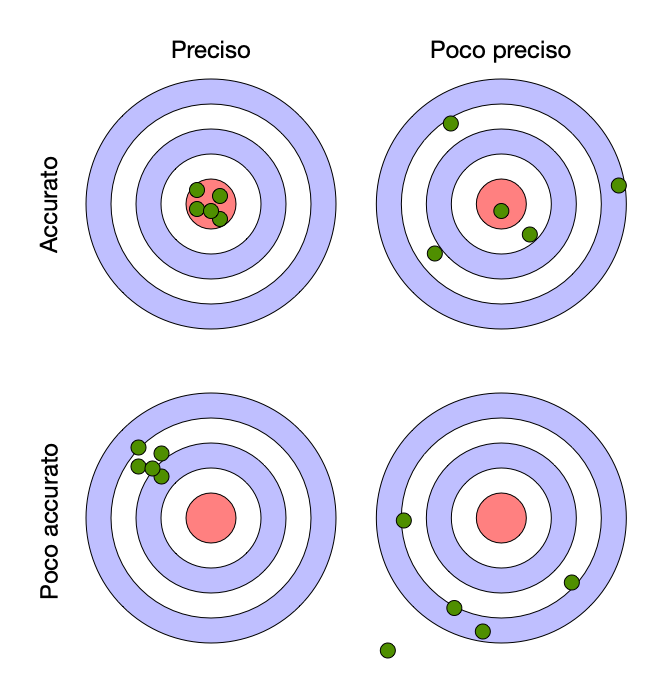
\includegraphics[width=5.20833in,height=\textheight,keepaspectratio]{images/bulls_eye.png}

\subsection{Norma UNI4546}\label{norma-uni4546}

Introdotta nel 1984, dà alcune \textbf{definizioni}:

Definizioni

\begin{itemize}
\tightlist
\item
  \textbf{Misurazione}: l'atto del misurare, assegnare valori numerici a
  grandezze fisiche
\item
  \textbf{Parametro}: grandezza di un sistema fisico alla quale
  assegnare valori numerici
\item
  \textbf{Misurando}: un parametro sottoposto a misurazione
\item
  \textbf{Misura}: il risultato di una misurazione
\item
  \textbf{Metrologia}: disciplina che riguarda la \textbf{qualità} delle
  misure
\end{itemize}

\subsection{Norma UNI4546}\label{norma-uni4546-1}

Una \textbf{misura}, che è il risultato di una \textbf{misurazione},
rappresenta un parametro di un sistema considerato \textbf{in un
determinato stato}

È una terna costituita da:

\begin{enumerate}
\def\labelenumi{\arabic{enumi}.}
\tightlist
\item
  un {valore}
\item
  un'{incertezza}
\item
  un'\textbf{unità di misura}
\end{enumerate}

Ad esempio: la mia statura è {183}{±0.5}~\textbf{cm}

Esistono due tipi di grandezze:

\begin{itemize}
\tightlist
\item
  \textbf{estensive}, per cui vale la somma (lunghezze, correnti
  elettriche, velocità)
\item
  \textbf{intensive}, esprimono un ordine e non vale la somma
  (pressioni, temperatura)
\end{itemize}

\marginnote{\begin{footnotesize}

L'incertezza è parte integrante di una misura; senza incertezza la
misura non è valida

\end{footnotesize}}

\subsection{Norma UNI4546}\label{norma-uni4546-2}

\begin{itemize}
\tightlist
\item
  Misurazione \textbf{diretta}: ottenuta per confronto diretto con un
  campione noto
\item
  Misurazione \textbf{indiretta}: si misurano grandezze secondarie
  collegate a quella di interesse mediante un \textbf{modello}
\end{itemize}

Nel caso di misurazione indiretta, lo strumento di misura è basato su un
\textbf{trasduttore}: un dispositivo che trasforma una grandezza fisica
in ingresso in un'altra grandezza (es. forza in carica elettrica)

Un \textbf{modello} è un insieme di relazioni tra parametri descrivente
le interazioni (m. \textbf{statico}) e possibilmente l'evoluzione nel
tempo (m. {dinamico}) di un sistema

Un modello può essere \textbf{analitico} o \textbf{numerico}

\marginnote{\begin{footnotesize}

Il modello di misura deve essere costruito sulla base della misura
stessa: non deve essere necessariamente esaustivo né basato sulla
comprensione fisica del sistema (cioè può anche essere
\textbf{empirico})

\end{footnotesize}}

\subsection{Norma GUM (ISO/IEC
98-3:2008)}\label{norma-gum-isoiec-98-32008}

\textbf{\emph{Guide to the expression of Uncertainty in Measurement}} è
il riferimento normativo per la terminologia e i metodi di calcolo
dell'incertezza nelle misurazioni

Secondo la GUM il risultato di una misurazione è una \textbf{variabile
aleatoria} e va trattato in quanto tale

La GUM ha abolito i termini di \textbf{errore} (sostituito con
{incertezza}) e di \textbf{valore vero} (sostituito con {stima})

Cioè si assume che il valore vero di una grandezza \textbf{non sia
conoscibile}: anche aumentando all'infinito la precisione di uno
strumento, prima o poi si arriva a livello atomico, per cui vale il
\textbf{principio di indeterminazione di Pauli}

Quindi, se non ha senso parlare di valore vero, allora non ha senso
nemmeno parlare di errore di misura

\subsection{Norma GUM (ISO/IEC
98-3:2008)}\label{norma-gum-isoiec-98-32008-1}

La GUM definisce:

Definizioni

\begin{itemize}
\tightlist
\item
  L'\textbf{incertezza standard} (\emph{standard uncertainty}) \(u_x\)
  della variabile \(x\) come la deviazione standard del valor medio di
  \(x\): \[
  u_x=\frac{s_x}{\sqrt{n}}=\sqrt{\frac{\sum_{i=1}^n(x_i-\bar x)^2}{n(n-1)}}
  \]
\item
  L'\textbf{incertezza relativa} come rapporto tra l'incertezza standard
  e la media della variabile; è adimensionale e utile per confronti: \[
  u_{x\mathrm{rel}}=\frac{u_x}{|\bar x|}
  \]
\end{itemize}

\subsection{Incertezza standard}\label{incertezza-standard}

l'\textbf{incertezza standard} può essere valutata

\begin{itemize}
\tightlist
\item
  mediante metodi statistici, come alla pagina precedente: in questo
  caso si parla di incertezza standard di \textbf{tipo A}
\item
  mediante l'uso di tutte le informazioni rilevanti possibili:
  incertezza standard di \textbf{tipo B}; essa è preferibile quando non
  si disponga di campione sufficiente di misure
\end{itemize}

Per \textbf{informazioni rilevanti} si intende ad esempio:

\begin{itemize}
\tightlist
\item
  dati di precedenti misurazioni
\item
  specifiche tecniche del costruttore dello strumento
\item
  certificati di taratura
\item
  esperienza o conoscenza generale degli strumenti di interesse
\end{itemize}

\subsection{Norma GUM (ISO/IEC
98-3:2008)}\label{norma-gum-isoiec-98-32008-2}

Definizioni

Ricordando che l'\textbf{intervallo di confidenza} è definito come \[
P\left(-t_{n-1,\alpha/2}\leq\frac{|\bar x - \mu_0|}{s_x/\sqrt{n}}\leq t_{n-1,\alpha/2}\right) = 1-\alpha
\] risulta che l'intervallo \(\bar x \pm t_{\alpha/2,n-1}u_x\) contiene
il valore atteso di \(x\) con una confidenza \(1-\alpha\)

Quindi la GUM definisce anche:

\begin{itemize}
\tightlist
\item
  L'\textbf{incertezza estesa} come la semi-ampiezza dell'intervallo di
  confidenza su \(\bar x\):
\end{itemize}

\[
U_x=t_{\alpha/2,n-1}\frac{s_x}{\sqrt{n}}=t_{\alpha/2,n-1}u_x = k_{n-1}u_x
\]

Il termine \(k_{n-1}\) è chiamato \textbf{fattore di copertura}, e
dipende solo dalla dimensione del campione (è il quantile della
distribuzione T di Student).

\subsection{Fattore di copertura}\label{fattore-di-copertura}

\textbf{Ricordare} che per \(n>50\) i quantili della normale e della T
di Student sono indistinguibili a livello pratico

Per questo motivo, per campioni sufficientemente grandi la GUM consente
di adottare i fattori di copertura ricavati dai quantili di
\(\mathcal{N}(0,1)\)

Salvo indicazioni, per esprimere una misura si usa sempre
l'\textbf{incertezza standard} (27.5±0.1mm, in cui \(u_x=0.1\))

\begin{Shaded}
\begin{Highlighting}[]
\FunctionTok{tibble}\NormalTok{(}
  \AttributeTok{conf=}\FunctionTok{c}\NormalTok{(}\FloatTok{0.6827}\NormalTok{, }\FloatTok{0.9}\NormalTok{, }\FloatTok{0.95}\NormalTok{, }\FloatTok{0.9545}\NormalTok{, }\FloatTok{0.99}\NormalTok{, }\FloatTok{0.9973}\NormalTok{),}
  \AttributeTok{alpha =} \DecValTok{1}\SpecialCharTok{{-}}\NormalTok{conf,}
  \AttributeTok{k=}\FunctionTok{qnorm}\NormalTok{(alpha}\SpecialCharTok{/}\DecValTok{2}\NormalTok{, }\AttributeTok{lower.tail =}\NormalTok{ F)}
\NormalTok{) }\SpecialCharTok{\%\textgreater{}\%} 
  \FunctionTok{mutate}\NormalTok{(}\AttributeTok{conf =} \FunctionTok{paste0}\NormalTok{(}\FunctionTok{as.character}\NormalTok{(conf}\SpecialCharTok{*}\DecValTok{100}\NormalTok{), }\StringTok{"\%"}\NormalTok{)) }\SpecialCharTok{\%\textgreater{}\%} 
\NormalTok{  knitr}\SpecialCharTok{::}\FunctionTok{kable}\NormalTok{(}\AttributeTok{col.names=}\FunctionTok{c}\NormalTok{(}\StringTok{"Livello di confidenza"}\NormalTok{, }
                           \StringTok{"$}\SpecialCharTok{\textbackslash{}\textbackslash{}}\StringTok{alpha$"}\NormalTok{,  }
                           \StringTok{"Fattore di copertura"}\NormalTok{),}
               \AttributeTok{align=}\FunctionTok{c}\NormalTok{(}\StringTok{"r"}\NormalTok{, }\StringTok{"r"}\NormalTok{, }\StringTok{"r"}\NormalTok{),}
               \AttributeTok{digits=}\DecValTok{4}\NormalTok{)}
\end{Highlighting}
\end{Shaded}

{\def\LTcaptype{none} % do not increment counter
\begin{longtable}[]{@{}rrr@{}}
\toprule\noalign{}
Livello di confidenza & \(\alpha\) & Fattore di copertura \\
\midrule\noalign{}
\endhead
\bottomrule\noalign{}
\endlastfoot
68.27\% & 0.3173 & 1.0000 \\
90\% & 0.1000 & 1.6449 \\
95\% & 0.0500 & 1.9600 \\
95.45\% & 0.0455 & 2.0000 \\
99\% & 0.0100 & 2.5758 \\
99.73\% & 0.0027 & 3.0000 \\
\end{longtable}
}

Se si usa l'\textbf{incertezza estesa} è necessario accompagnarla dal
\textbf{livello di confidenza} (27.5±0.1mm al 95\%)

\marginnote{\begin{footnotesize}

Per campioni con meno di 50 elementi è opportuno calcolare il fattore di
copertura come \(t_{\alpha/2,n-1}\)

\end{footnotesize}}

\subsection{Modello statico di uno strumento di
misura}\label{modello-statico-di-uno-strumento-di-misura}

Nel caso di \textbf{misurazioni indirette}, è fondamentale disporre di
un modello che descriva il comportamento del trasduttore, cioè la
relazione tra uscita e ingresso

Ogni modello dipende da uno o più parametri numerici che devono essere
identificati

Questa operazione di identificazione dei parametri del modello di misura
si chiama \textbf{taratura}

La taratura punta a definire la correlazione \(y=f(m)\) tra l'ingresso
misurando \(m\) e l'uscita del trasduttore \(y\), e la relativa
\textbf{incertezza}. La \(f(\cdot)\) è detta \textbf{caratteristica
statica dello strumento}

D'ora in avanti considereremo solo il caso di \textbf{sistemi statici},
cioè in stato stazionario, per i quali \textbf{il tempo non è una
variabile di modello}

I \textbf{sistemi dinamici} verranno presi in considerazione nel secondo
modulo di questo corso

\marginnote{\begin{footnotesize}

Si parla di \textbf{taratura statica o dinamica} per una operazione di
misurazione statica o dinamica, rispettivamente

\end{footnotesize}}

\subsection{Taratura}\label{taratura}

Uno strumento fornisce la misura mediante \textbf{inversione della
caratteristica statica}: \(m=f^{-1}(y)\)

Perché la \(f(\cdot)\) sia nota è necessario identificarne i parametri
mediante \textbf{regressione}

La regressione viene effettuata a partire da una serie di coppie
\((m_i, y_i)\) ottenute:

\begin{itemize}
\tightlist
\item
  da una serie di \textbf{misurandi noti} \(m_i\)
\item
  da una serie di misurazioni \(y_i\) ottenute con uno strumento di
  qualità migliore di quello in taratura
\end{itemize}

\subsubsection{Misurazione}

\begin{Shaded}
\begin{Highlighting}[]
\NormalTok{df }\OtherTok{\textless{}{-}} \FunctionTok{tibble}\NormalTok{(}
  \AttributeTok{i=}\DecValTok{1}\SpecialCharTok{:}\DecValTok{100}\NormalTok{,}
  \AttributeTok{x=}\FunctionTok{seq}\NormalTok{(}\DecValTok{0}\NormalTok{,}\DecValTok{10}\NormalTok{,}\AttributeTok{length.out=}\FunctionTok{length}\NormalTok{(i)),}
  \AttributeTok{y=}\FunctionTok{sqrt}\NormalTok{(x),}
  \AttributeTok{s=}\NormalTok{F}
\NormalTok{)}
\NormalTok{df[df}\SpecialCharTok{$}\NormalTok{i}\SpecialCharTok{\%\%}\DecValTok{10}\SpecialCharTok{==}\DecValTok{0}\NormalTok{,]}\SpecialCharTok{$}\NormalTok{s }\OtherTok{\textless{}{-}}\NormalTok{ T}

\NormalTok{p1 }\OtherTok{\textless{}{-}}\NormalTok{ df }\SpecialCharTok{\%\textgreater{}\%} \FunctionTok{ggplot}\NormalTok{(}\FunctionTok{aes}\NormalTok{(}\AttributeTok{x=}\NormalTok{x, }\AttributeTok{y=}\NormalTok{y)) }\SpecialCharTok{+} 
  \FunctionTok{geom\_line}\NormalTok{() }\SpecialCharTok{+} 
  \FunctionTok{labs}\NormalTok{(}\AttributeTok{x=}\StringTok{"misurando (ignoto)"}\NormalTok{, }\AttributeTok{y=}\StringTok{"uscita osservata"}\NormalTok{)}

\NormalTok{point }\OtherTok{\textless{}{-}} \FunctionTok{filter}\NormalTok{(df, i}\SpecialCharTok{==}\DecValTok{30}\NormalTok{)}
\NormalTok{arw }\OtherTok{\textless{}{-}} \FunctionTok{arrow}\NormalTok{(}\AttributeTok{angle=}\DecValTok{20}\NormalTok{, }\AttributeTok{type=}\StringTok{"closed"}\NormalTok{, }\AttributeTok{length=}\FunctionTok{unit}\NormalTok{(}\FloatTok{0.2}\NormalTok{, }\StringTok{"inches"}\NormalTok{))}
\NormalTok{p1 }\SpecialCharTok{+}
  \FunctionTok{geom\_segment}\NormalTok{(}\AttributeTok{xend=}\NormalTok{point}\SpecialCharTok{$}\NormalTok{x, }\AttributeTok{yend=}\DecValTok{0}\NormalTok{, }\AttributeTok{x=}\NormalTok{point}\SpecialCharTok{$}\NormalTok{x, }\AttributeTok{y=}\NormalTok{point}\SpecialCharTok{$}\NormalTok{y, }\AttributeTok{arrow=}\NormalTok{arw, }\AttributeTok{color=}\FunctionTok{gray}\NormalTok{(}\FloatTok{0.5}\NormalTok{)) }\SpecialCharTok{+}
  \FunctionTok{geom\_segment}\NormalTok{(}\AttributeTok{xend=}\NormalTok{point}\SpecialCharTok{$}\NormalTok{x, }\AttributeTok{yend=}\NormalTok{point}\SpecialCharTok{$}\NormalTok{y, }\AttributeTok{x=}\DecValTok{0}\NormalTok{, }\AttributeTok{y=}\NormalTok{point}\SpecialCharTok{$}\NormalTok{y, }\AttributeTok{arrow=}\NormalTok{arw, }\AttributeTok{color=}\FunctionTok{gray}\NormalTok{(}\FloatTok{0.5}\NormalTok{)) }\SpecialCharTok{+} 
  \FunctionTok{geom\_point}\NormalTok{(}\AttributeTok{data=}\NormalTok{point, }\AttributeTok{size=}\DecValTok{3}\NormalTok{, }\AttributeTok{color=}\StringTok{"black"}\NormalTok{, }\AttributeTok{fill=}\StringTok{"blue"}\NormalTok{, }\AttributeTok{shape=}\DecValTok{21}\NormalTok{)}
\end{Highlighting}
\end{Shaded}

\pandocbounded{\includegraphics[keepaspectratio]{5-misura_files/figure-pdf/unnamed-chunk-3-1.pdf}}

\subsubsection{Taratura}

\begin{Shaded}
\begin{Highlighting}[]
\NormalTok{point }\OtherTok{\textless{}{-}} \FunctionTok{filter}\NormalTok{(df, i}\SpecialCharTok{==}\DecValTok{30}\NormalTok{)}
\NormalTok{p1 }\SpecialCharTok{+}
  \FunctionTok{geom\_segment}\NormalTok{(}\AttributeTok{x=}\NormalTok{point}\SpecialCharTok{$}\NormalTok{x, }\AttributeTok{y=}\DecValTok{0}\NormalTok{, }\AttributeTok{xend=}\NormalTok{point}\SpecialCharTok{$}\NormalTok{x, }\AttributeTok{yend=}\NormalTok{point}\SpecialCharTok{$}\NormalTok{y, }\AttributeTok{arrow=}\NormalTok{arw, }\AttributeTok{color=}\FunctionTok{gray}\NormalTok{(}\FloatTok{0.5}\NormalTok{)) }\SpecialCharTok{+}
  \FunctionTok{geom\_segment}\NormalTok{(}\AttributeTok{xend=}\NormalTok{point}\SpecialCharTok{$}\NormalTok{x, }\AttributeTok{yend=}\NormalTok{point}\SpecialCharTok{$}\NormalTok{y, }\AttributeTok{x=}\DecValTok{0}\NormalTok{, }\AttributeTok{y=}\NormalTok{point}\SpecialCharTok{$}\NormalTok{y, }\AttributeTok{arrow=}\NormalTok{arw, }\AttributeTok{color=}\FunctionTok{gray}\NormalTok{(}\FloatTok{0.5}\NormalTok{)) }\SpecialCharTok{+} 
  \FunctionTok{geom\_point}\NormalTok{(}\AttributeTok{data=}\FunctionTok{filter}\NormalTok{(df, s), }\AttributeTok{size=}\DecValTok{3}\NormalTok{, }\AttributeTok{color=}\StringTok{"black"}\NormalTok{, }\AttributeTok{fill=}\StringTok{"blue"}\NormalTok{, }\AttributeTok{shape=}\DecValTok{21}\NormalTok{) }\SpecialCharTok{+}
  \FunctionTok{labs}\NormalTok{(}\AttributeTok{x=}\StringTok{"misurando (noto)"}\NormalTok{, }\AttributeTok{y=}\StringTok{"uscita osservata"}\NormalTok{)}
\end{Highlighting}
\end{Shaded}

\pandocbounded{\includegraphics[keepaspectratio]{5-misura_files/figure-pdf/unnamed-chunk-4-1.pdf}}

\marginnote{\begin{footnotesize}

Per ``strumento migliore'' si intende uno strumento con una precisione
migliore di almeno un ordine di grandezza

\end{footnotesize}}

\subsection{Taratura}\label{taratura-2}

Una \textbf{taratura statica} si sviluppa quindi su quattro passaggi:

\begin{enumerate}
\def\labelenumi{\arabic{enumi}.}
\tightlist
\item
  \textbf{sviluppo del modello dello strumento}: mediante analisi dei
  principi fisici si definisce la caratteristica statica come relazione
  (analitica, numerica o mista) tra ingresso e uscita. Idealmente, un
  modello completo comprende anche gli \textbf{ingressi di disturbo}
\item
  \textbf{raccolta dei dati di taratura}: una campagna sperimentale
  fornisce le coppie \((m_i, y_i)\), che \textbf{vanno raccolte con
  \(m\) in ordine casuale}
\item
  \textbf{regressione}: si identificano i parametri del modello
\item
  \textbf{validazione del modello}: si verifica l'adeguatezza del
  modello regredito mediante analisi dei residui
\end{enumerate}

La taratura deve anche definire l'\textbf{incertezza} dello strumento,
dovuta:

\begin{itemize}
\tightlist
\item
  al modello (la \emph{forma} della caratteristica statica)
\item
  ai parametri del modello
\item
  alla stima del misurando (dovuta a ingressi di disturbo)
\end{itemize}

\subsection{Ingressi di disturbo}\label{ingressi-di-disturbo}

Gli ingressi fonte di incertezza possono essere:

\begin{itemize}
\tightlist
\item
  \textbf{ingressi modificanti}: modificano la caratteristica statica,
  per cui ad uno stesso valore di \(m\) possono corrispondere diversi
  valori di \(y\) per via di un cambiamento della \textbf{forma} di
  \(f(\cdot)\) o del valore dei parametri (ad es. effetto della
  temperatura)
\item
  \textbf{ingressi interferenti}: si sommano direttamente all'uscita
  dello strumento, per cui \(y=f(m)+y_d\), e hanno tipicamente un
  carattere stocastico (ad es. vibrazioni, disturbi elettrici)
\end{itemize}

\pandocbounded{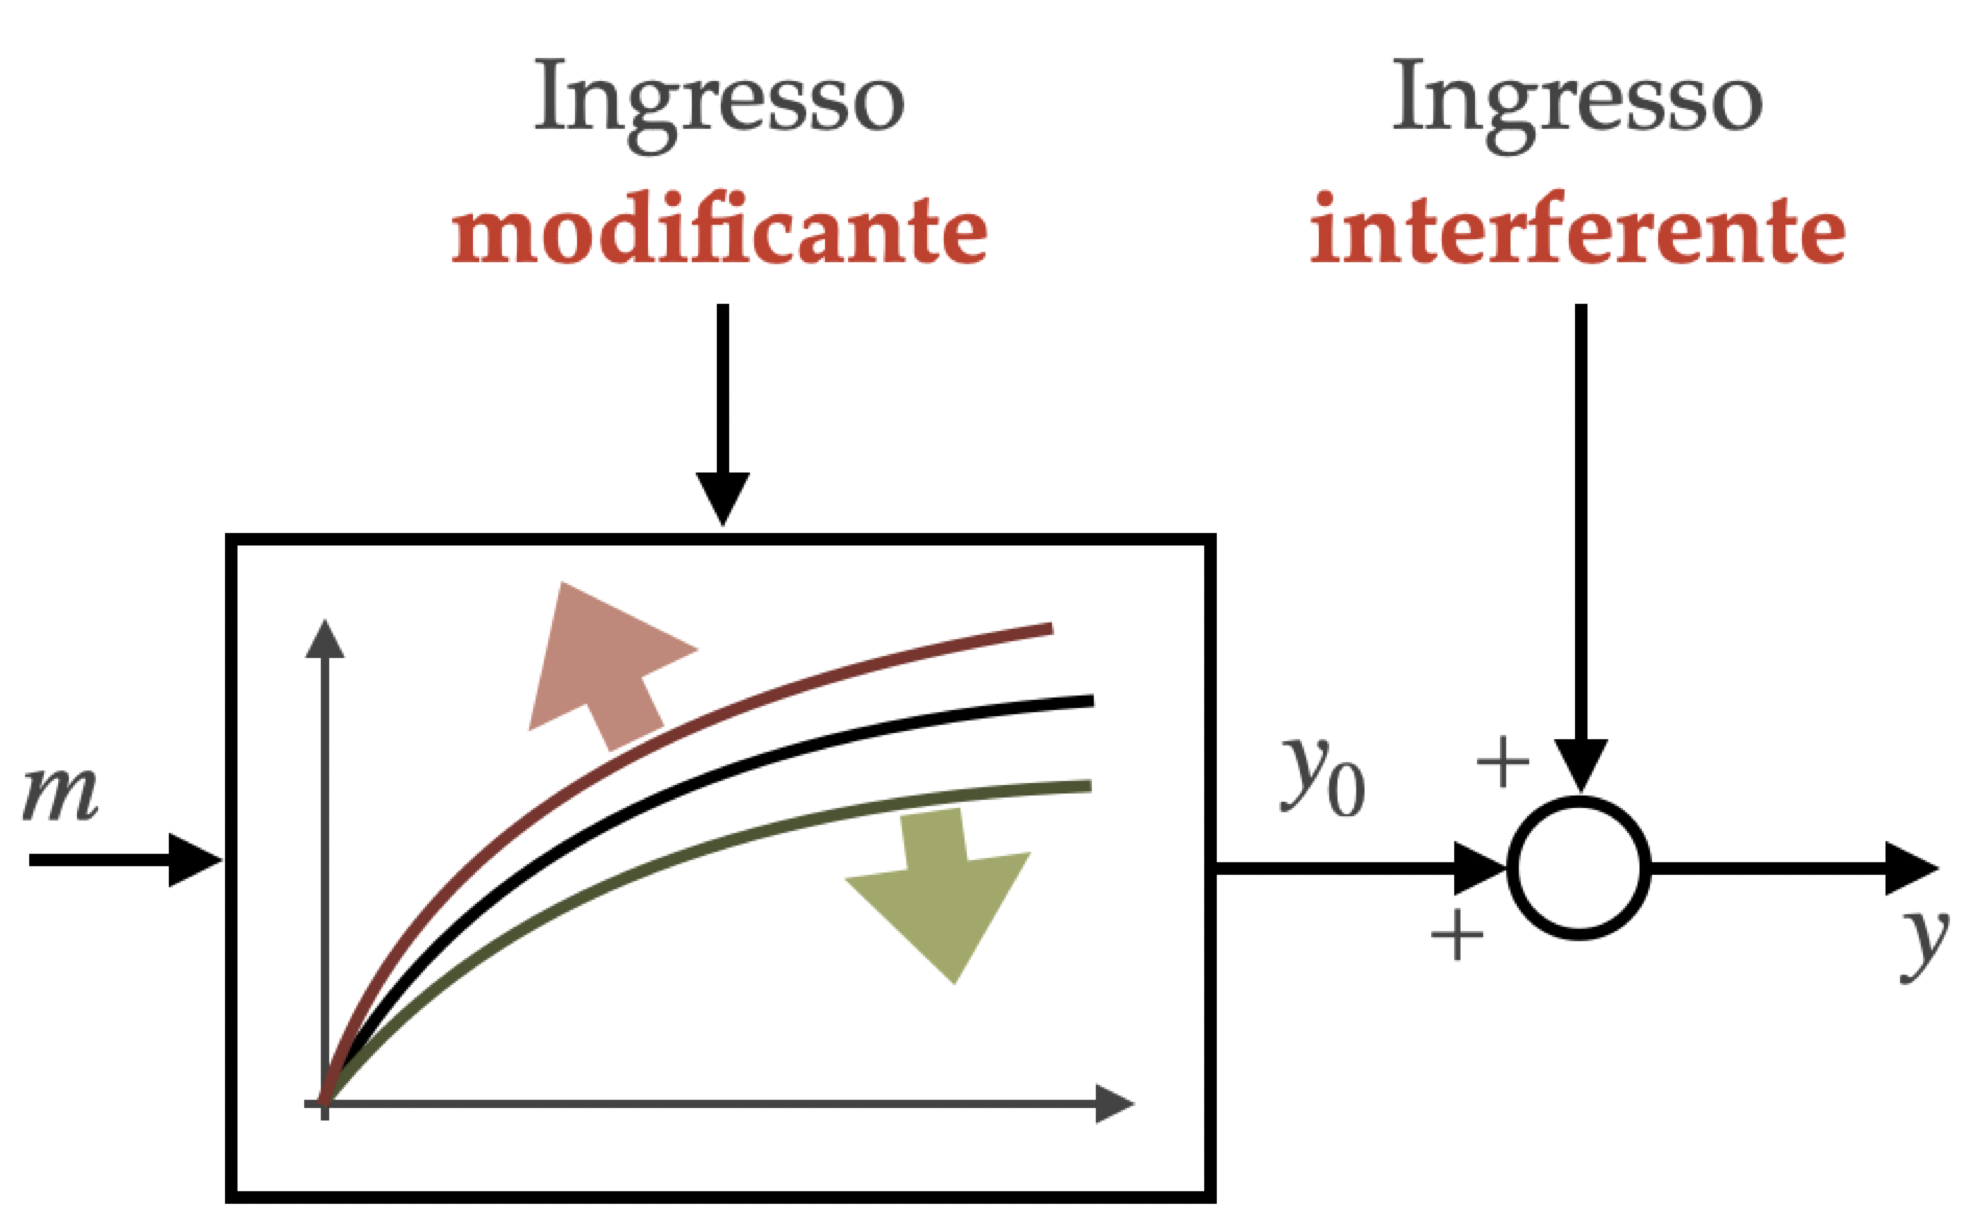
\includegraphics[keepaspectratio]{images/modellomisura.png}}

\marginnote{\begin{footnotesize}

L'incertezza si riferisce solo alla componente aleatoria e non
prevedibile della misura; si assume che ogni componente di deviazione
sistematica sia già stato corretto

\end{footnotesize}}

\subsection{Esempio: dinamometro a
mensola}\label{esempio-dinamometro-a-mensola}

È uno strumento per la misura della \textbf{forza peso} che sfrutta:

\begin{itemize}
\tightlist
\item
  l'elasticità di una trave snella per convertire una forza in una
  deformazione
\item
  un estensimetro per convertire una deformazione in una variazione di
  resistenza
\item
  un circuito elettrico con voltmetro per convertire la variazione di
  resistenza in variazione di corrente, mediante \textbf{amplificazione}
\end{itemize}

Il modello dello strumento fornisce:

\subsubsection{Dinamometro}

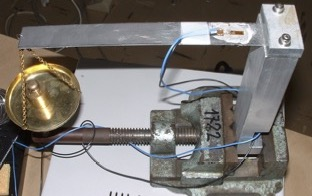
\includegraphics[width=5.20833in,height=\textheight,keepaspectratio]{images/cantilever.jpg}

\subsubsection{Amplificatore}

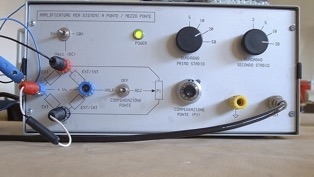
\includegraphics[width=5.20833in,height=\textheight,keepaspectratio]{images/amplifier.jpg}

\[
V=3/2GV_i\frac{lG_F}{EBH^2}F+V_0 = V_0+ KF
\]

\subsection{Esempio: dinamometro a
mensola}\label{esempio-dinamometro-a-mensola-1}

La caratteristica statica dello strumento dipende, oltre che dal
misurando \(F\), da altri 8 parametri

Per effettuare la taratura si tengono il più possibile costanti tutti i
parametri, eccetto il misurando

I parametri che non è possibile mantenere costanti si accetta che
fluttuino, ripetendo le misurazioni e mediando i risultati: si parla di
\textbf{controllo statistico del processo di taratura}, che mitiga
l'effetto degli \textbf{ingressi interferenti}

È la condizione in cui si applica il \textbf{teorema del limite
centrale}

Gli \textbf{ingressi modificanti} sono più complessi da trattare e
richiedono una modifica del modello e il passaggio da uno strumento di
misura a un \textbf{sistema di misura}

Ad esempio, \textbf{la temperatura} può influire su tutti i parametri
della caratteristica statica: se affianco uno strumento di misura della
temperatura e arricchisco il modello con la dipendenza dalla
temperatura, posso \textbf{compensare l'effetto} degli ingressi
modificanti

\marginnote{\begin{footnotesize}

Un \textbf{sistema di misura} è costituito da più strumenti che lavorano
assieme

\end{footnotesize}}

\subsection{Casualizzazione della sequenza di
taratura}\label{casualizzazione-della-sequenza-di-taratura}

Compensare l'effetto degli ingressi modificanti durante la taratura può
non essere semplice o economico

Se però raccolgo le coppie \((m_y, y_i)\) in ordine casuale anziché in
ordine di \(m_i\), ottengo il risultato di \textbf{distribuire
casualmente} l'effetto degli ingressi modificanti

In questo modo trasformo gli ingressi modificanti in \textbf{ingressi
interferenti}, dei quali posso mitigare l'effetto mediante
\textbf{controllo statistico}

Confrontiamo ora la taratura del dinamometro a mensola effettuata
\textbf{senza casualizzazione} e {con casualizzazione}, nel caso di un
ingresso modificante (la temperatura) non preso in considerazione
dall'operatore

\subsection{Taratura del dinamometro (senza
casualizzazione)}\label{taratura-del-dinamometro-senza-casualizzazione}

Nel laboratorio di taratura, dopo 4 ore dall'inizio del processo di
taratura, il termostato viene modificato e la temperatura comincia a
variare tra 20°C e 25°C

L'addetto alla calibrazione \textbf{non si accorge} del cambiamento
\textbf{né registra la temperatura}

\begin{Shaded}
\begin{Highlighting}[]
\FunctionTok{set.seed}\NormalTok{(}\DecValTok{120}\NormalTok{)}
\NormalTok{parameters }\OtherTok{\textless{}{-}} \FunctionTok{list}\NormalTok{(}
  \AttributeTok{G=}\DecValTok{10}\NormalTok{,}
  \AttributeTok{Vi=}\DecValTok{12}\NormalTok{,}
  \AttributeTok{l=}\DecValTok{300}\NormalTok{,}
  \AttributeTok{E=}\DecValTok{200}\NormalTok{,}
  \AttributeTok{B=}\DecValTok{20}\NormalTok{,}
  \AttributeTok{H=}\DecValTok{2}\NormalTok{,}
  \AttributeTok{V0=}\DecValTok{1}
\NormalTok{)}
\NormalTok{Gf }\OtherTok{\textless{}{-}} \ControlFlowTok{function}\NormalTok{(Temp, }\AttributeTok{G0=}\FloatTok{0.05}\NormalTok{, }\AttributeTok{T0=}\DecValTok{20}\NormalTok{, }\AttributeTok{k=}\FloatTok{0.01}\NormalTok{) G0 }\SpecialCharTok{+}\NormalTok{ k}\SpecialCharTok{*}\NormalTok{(Temp}\SpecialCharTok{{-}}\NormalTok{T0) }
\NormalTok{K }\OtherTok{\textless{}{-}} \ControlFlowTok{function}\NormalTok{(Temp, params) }\FunctionTok{with}\NormalTok{(params, }\DecValTok{3}\SpecialCharTok{/}\DecValTok{2}\SpecialCharTok{*}\NormalTok{G}\SpecialCharTok{*}\NormalTok{Vi}\SpecialCharTok{*}\NormalTok{(l}\SpecialCharTok{*}\FunctionTok{Gf}\NormalTok{(Temp))}\SpecialCharTok{/}\NormalTok{(E}\SpecialCharTok{*}\NormalTok{B}\SpecialCharTok{*}\NormalTok{H}\SpecialCharTok{\^{}}\DecValTok{2}\NormalTok{))}
\NormalTok{model }\OtherTok{\textless{}{-}} \ControlFlowTok{function}\NormalTok{(F, Temp, params) }\FunctionTok{K}\NormalTok{(Temp, params) }\SpecialCharTok{*}\NormalTok{ F }\SpecialCharTok{+}\NormalTok{ params}\SpecialCharTok{$}\NormalTok{V0}
\NormalTok{temp }\OtherTok{\textless{}{-}} \ControlFlowTok{function}\NormalTok{(time, }\AttributeTok{t0=}\DecValTok{4}\NormalTok{, }\AttributeTok{T0=}\DecValTok{20}\NormalTok{, }\AttributeTok{dT=}\DecValTok{5}\NormalTok{, }\AttributeTok{tau=}\DecValTok{2}\NormalTok{) }\FunctionTok{ifelse}\NormalTok{(time}\SpecialCharTok{\textless{}}\NormalTok{t0, T0, T0}\SpecialCharTok{+}\NormalTok{dT}\SpecialCharTok{*}\NormalTok{(}\DecValTok{1}\SpecialCharTok{{-}}\FunctionTok{exp}\NormalTok{(}\SpecialCharTok{{-}}\NormalTok{(time}\SpecialCharTok{{-}}\NormalTok{t0)}\SpecialCharTok{/}\NormalTok{tau)))}
\NormalTok{N }\OtherTok{\textless{}{-}} \DecValTok{50}
\NormalTok{duration }\OtherTok{\textless{}{-}} \DecValTok{8}
\NormalTok{data }\OtherTok{\textless{}{-}} \FunctionTok{tibble}\NormalTok{(}
  \AttributeTok{t =} \FunctionTok{seq}\NormalTok{(}\DecValTok{0}\NormalTok{, duration, }\AttributeTok{length.out=}\NormalTok{N),}
  \AttributeTok{Temp =} \FunctionTok{temp}\NormalTok{(t),}
  \AttributeTok{Gf =} \FunctionTok{Gf}\NormalTok{(Temp),}
  \AttributeTok{Force =} \FunctionTok{seq}\NormalTok{(}\DecValTok{10}\NormalTok{, }\DecValTok{100}\NormalTok{, }\AttributeTok{length.out=}\NormalTok{N),}
  \AttributeTok{Vn =} \FunctionTok{model}\NormalTok{(Force, Temp, parameters),}
  \AttributeTok{V=}\NormalTok{Vn}\SpecialCharTok{+}\FunctionTok{rnorm}\NormalTok{(}\FunctionTok{length}\NormalTok{(t), }\DecValTok{0}\NormalTok{, }\FloatTok{0.5}\NormalTok{)}
\NormalTok{)}
\NormalTok{data.lm }\OtherTok{\textless{}{-}} \FunctionTok{lm}\NormalTok{(V}\SpecialCharTok{\textasciitilde{}}\NormalTok{Force, }\AttributeTok{data=}\NormalTok{data)}
\NormalTok{data }\OtherTok{\textless{}{-}} \FunctionTok{add\_predictions}\NormalTok{(data, data.lm, }\AttributeTok{var=}\StringTok{"pred.nr1"}\NormalTok{)}
\NormalTok{data }\OtherTok{\textless{}{-}} \FunctionTok{add\_residuals}\NormalTok{(data, }\AttributeTok{model=}\NormalTok{data.lm, }\AttributeTok{var=}\StringTok{"res.nr1"}\NormalTok{)}
\end{Highlighting}
\end{Shaded}

\begin{Shaded}
\begin{Highlighting}[]
\FunctionTok{tibble}\NormalTok{(}\AttributeTok{x=}\FunctionTok{seq}\NormalTok{(}\DecValTok{0}\NormalTok{, }\DecValTok{20}\NormalTok{, }\AttributeTok{length.out=}\DecValTok{100}\NormalTok{)) }\SpecialCharTok{\%\textgreater{}\%} \FunctionTok{ggplot}\NormalTok{(}\FunctionTok{aes}\NormalTok{(x)) }\SpecialCharTok{+}
  \FunctionTok{geom\_function}\NormalTok{(}\AttributeTok{fun=}\NormalTok{temp) }\SpecialCharTok{+}
  \FunctionTok{labs}\NormalTok{(}\AttributeTok{x=}\StringTok{"Tempo (h)"}\NormalTok{, }\AttributeTok{y=}\StringTok{"Temperatura (°C)"}\NormalTok{)}
\end{Highlighting}
\end{Shaded}

\pandocbounded{\includegraphics[keepaspectratio]{5-misura_files/figure-pdf/unnamed-chunk-6-1.pdf}}

\subsection{Taratura del dinamometro (senza
casualizzazione)}\label{taratura-del-dinamometro-senza-casualizzazione-1}

L'addetto registra la tensione in uscita in corrispondenza di 50 valori
di forza applicati, variabili tra 10~N e 100~N, \textbf{in ordine
crescente della forza}

Dato che il modello dello strumento prevede una relazione lineare
\(V=V_0+KF\), l'addetto effettua una regressione lineare

Lo studio dei residui però evidenzia un \emph{pattern} con un minimo,
per cui l'addetto \textbf{sospetta un sotto-adattamento} e quindi tenta
una seconda regressione con un modello quadratico

\subsubsection{Regressione}

\begin{Shaded}
\begin{Highlighting}[]
\NormalTok{data }\SpecialCharTok{\%\textgreater{}\%} \FunctionTok{ggplot}\NormalTok{(}\FunctionTok{aes}\NormalTok{(}\AttributeTok{x=}\NormalTok{Force)) }\SpecialCharTok{+}
  \FunctionTok{geom\_point}\NormalTok{(}\FunctionTok{aes}\NormalTok{(}\AttributeTok{y=}\NormalTok{V)) }\SpecialCharTok{+} 
  \FunctionTok{geom\_hline}\NormalTok{(}\AttributeTok{yintercept=}\NormalTok{parameters}\SpecialCharTok{$}\NormalTok{V0, }\AttributeTok{linetype=}\DecValTok{2}\NormalTok{) }\SpecialCharTok{+}
  \FunctionTok{geom\_line}\NormalTok{(}\FunctionTok{aes}\NormalTok{(}\AttributeTok{y=}\NormalTok{pred.nr1), }\AttributeTok{color=}\StringTok{"red"}\NormalTok{) }\SpecialCharTok{+}
  \FunctionTok{labs}\NormalTok{(}\AttributeTok{x=}\StringTok{"Forza (N)"}\NormalTok{, }\AttributeTok{y=}\StringTok{"Tensione (V)"}\NormalTok{)}
\end{Highlighting}
\end{Shaded}

\pandocbounded{\includegraphics[keepaspectratio]{5-misura_files/figure-pdf/unnamed-chunk-7-1.pdf}}

\subsubsection{Residui}

\begin{Shaded}
\begin{Highlighting}[]
\NormalTok{data }\SpecialCharTok{\%\textgreater{}\%}
  \FunctionTok{ggplot}\NormalTok{(}\FunctionTok{aes}\NormalTok{(}\AttributeTok{x=}\NormalTok{Force, }\AttributeTok{y=}\NormalTok{res.nr1)) }\SpecialCharTok{+}
  \FunctionTok{geom\_point}\NormalTok{() }\SpecialCharTok{+}
  \FunctionTok{labs}\NormalTok{(}\AttributeTok{x=}\StringTok{"Forza (N)"}\NormalTok{, }\AttributeTok{y=}\StringTok{"Residui (V)"}\NormalTok{)}
\end{Highlighting}
\end{Shaded}

\pandocbounded{\includegraphics[keepaspectratio]{5-misura_files/figure-pdf/unnamed-chunk-8-1.pdf}}

\subsection{Taratura del dinamometro (senza
casualizzazione)}\label{taratura-del-dinamometro-senza-casualizzazione-2}

L'addetto verifica quindi una regressione con un modello di secondo
grado

L'analisi dei residui lo soddisfa e quindi accetta la nuova
caratteristica statica tarata come un polinomio di secondo grado

\textbf{Nota}: questa caratteristica ha perso la relazione con la fisica
del problema ed è quindi \textbf{puramente empirica}

Tuttavia, dato che la variazione di temperatura \textbf{non è stata
registrata né notata}, l'addetto non ha modo di accorgersi che la
caratteristica così tarata è ovviamente sbagliata e in pratica
inutilizzabile

\subsubsection{Regressione}

\begin{Shaded}
\begin{Highlighting}[]
\NormalTok{data.lm2 }\OtherTok{\textless{}{-}} \FunctionTok{lm}\NormalTok{(V}\SpecialCharTok{\textasciitilde{}}\FunctionTok{poly}\NormalTok{(Force, }\AttributeTok{degree=}\DecValTok{2}\NormalTok{, }\AttributeTok{raw=}\NormalTok{T), }\AttributeTok{data=}\NormalTok{data)}
\NormalTok{data }\OtherTok{\textless{}{-}} \FunctionTok{add\_predictions}\NormalTok{(data, data.lm2, }\AttributeTok{var=}\StringTok{"pred.nr2"}\NormalTok{)}
\NormalTok{data }\OtherTok{\textless{}{-}} \FunctionTok{add\_residuals}\NormalTok{(data, }\AttributeTok{model=}\NormalTok{data.lm2, }\AttributeTok{var=}\StringTok{"res.nr2"}\NormalTok{)}

\NormalTok{data }\SpecialCharTok{\%\textgreater{}\%} \FunctionTok{ggplot}\NormalTok{(}\FunctionTok{aes}\NormalTok{(}\AttributeTok{x=}\NormalTok{Force)) }\SpecialCharTok{+}
  \FunctionTok{geom\_point}\NormalTok{(}\FunctionTok{aes}\NormalTok{(}\AttributeTok{y=}\NormalTok{V)) }\SpecialCharTok{+} 
  \FunctionTok{geom\_hline}\NormalTok{(}\AttributeTok{yintercept=}\NormalTok{parameters}\SpecialCharTok{$}\NormalTok{V0, }\AttributeTok{linetype=}\DecValTok{2}\NormalTok{) }\SpecialCharTok{+}
  \FunctionTok{geom\_line}\NormalTok{(}\FunctionTok{aes}\NormalTok{(}\AttributeTok{y=}\NormalTok{pred.nr2), }\AttributeTok{color=}\StringTok{"red"}\NormalTok{) }\SpecialCharTok{+}
  \FunctionTok{labs}\NormalTok{(}\AttributeTok{x=}\StringTok{"Forza (N)"}\NormalTok{, }\AttributeTok{y=}\StringTok{"Tensione (V)"}\NormalTok{)}
\end{Highlighting}
\end{Shaded}

\pandocbounded{\includegraphics[keepaspectratio]{5-misura_files/figure-pdf/unnamed-chunk-9-1.pdf}}

\subsubsection{Residui}

\begin{Shaded}
\begin{Highlighting}[]
\NormalTok{data }\SpecialCharTok{\%\textgreater{}\%}
  \FunctionTok{ggplot}\NormalTok{(}\FunctionTok{aes}\NormalTok{(}\AttributeTok{x=}\NormalTok{Force, }\AttributeTok{y=}\NormalTok{res.nr2)) }\SpecialCharTok{+}
  \FunctionTok{geom\_point}\NormalTok{() }\SpecialCharTok{+}
  \FunctionTok{labs}\NormalTok{(}\AttributeTok{x=}\StringTok{"Forza (N)"}\NormalTok{, }\AttributeTok{y=}\StringTok{"Residui (V)"}\NormalTok{)}
\end{Highlighting}
\end{Shaded}

\pandocbounded{\includegraphics[keepaspectratio]{5-misura_files/figure-pdf/unnamed-chunk-10-1.pdf}}

\marginnote{\begin{footnotesize}

I residui non sono del tutto privi di pattern (andamento a ``M'').
Tuttavia, aumentando il grado della regressione si può raggiungere un
livello (grado 6) in cui i residui sono effettivamente privi di pattern,
ma ciò tuttavia non invalida quanto sopra detto

\end{footnotesize}}

\subsection{\texorpdfstring{Taratura del dinamometro {(con
casualizzazione)}}{Taratura del dinamometro (con casualizzazione)}}\label{taratura-del-dinamometro-con-casualizzazione}

Rivediamo cosa sarebbe successo raccogliendo le coppie \((m_i,y_i)\) in
\textbf{ordine casuale}

In questo caso l'effetto di aumento della temperatura è nullo sulle
coppie raccolte (con valori casuali di \(m_i\)!) prima di 4 ore;
successivamente questo effetto si distribuisce casualmente su tutti i
valori del misurando (diventa un ingresso interferente)

La regressione lineare di primo grado questa volta è adatta, anche se la
varianza non è costante

Tuttavia, osservando i \textbf{residui in funzione del tempo} si nota
che a circa 4 ore inizia a succedere qualcosa che fa aumentare i residui

\subsubsection{Regressione}

\begin{Shaded}
\begin{Highlighting}[]
\FunctionTok{set.seed}\NormalTok{(}\DecValTok{120}\NormalTok{)}
\NormalTok{data }\OtherTok{\textless{}{-}}\NormalTok{ data }\SpecialCharTok{\%\textgreater{}\%} \FunctionTok{mutate}\NormalTok{(}
  \AttributeTok{Force =} \FunctionTok{sample}\NormalTok{(Force),}
  \AttributeTok{Vn =} \FunctionTok{model}\NormalTok{(Force, Temp, parameters),}
  \AttributeTok{V=}\NormalTok{Vn}\SpecialCharTok{+}\FunctionTok{rnorm}\NormalTok{(}\FunctionTok{length}\NormalTok{(t), }\DecValTok{0}\NormalTok{, }\FloatTok{0.5}\NormalTok{) }
\NormalTok{)}
\NormalTok{data.lm3 }\OtherTok{\textless{}{-}} \FunctionTok{lm}\NormalTok{(V}\SpecialCharTok{\textasciitilde{}}\NormalTok{Force, }\AttributeTok{data=}\NormalTok{data)}
\NormalTok{data }\OtherTok{\textless{}{-}} \FunctionTok{add\_predictions}\NormalTok{(data, data.lm3, }\AttributeTok{var=}\StringTok{"pred.r"}\NormalTok{)}
\NormalTok{data }\OtherTok{\textless{}{-}} \FunctionTok{add\_residuals}\NormalTok{(data, data.lm3, }\AttributeTok{var=}\StringTok{"res.r"}\NormalTok{)}

\NormalTok{data }\SpecialCharTok{\%\textgreater{}\%} \FunctionTok{ggplot}\NormalTok{(}\FunctionTok{aes}\NormalTok{(}\AttributeTok{x=}\NormalTok{Force)) }\SpecialCharTok{+}
  \FunctionTok{geom\_point}\NormalTok{(}\FunctionTok{aes}\NormalTok{(}\AttributeTok{y=}\NormalTok{V)) }\SpecialCharTok{+} 
  \FunctionTok{geom\_line}\NormalTok{(}\FunctionTok{aes}\NormalTok{(}\AttributeTok{y=}\NormalTok{pred.r), }\AttributeTok{color=}\StringTok{"red"}\NormalTok{) }\SpecialCharTok{+}
  \FunctionTok{geom\_hline}\NormalTok{(}\AttributeTok{yintercept=}\NormalTok{parameters}\SpecialCharTok{$}\NormalTok{V0, }\AttributeTok{linetype=}\DecValTok{2}\NormalTok{) }\SpecialCharTok{+}
  \FunctionTok{labs}\NormalTok{(}\AttributeTok{x=}\StringTok{"Forza (N)"}\NormalTok{, }\AttributeTok{y=}\StringTok{"Tensione (V)"}\NormalTok{)}
\end{Highlighting}
\end{Shaded}

\pandocbounded{\includegraphics[keepaspectratio]{5-misura_files/figure-pdf/unnamed-chunk-11-1.pdf}}

\subsubsection{Residui (F)}

\begin{Shaded}
\begin{Highlighting}[]
\NormalTok{data }\SpecialCharTok{\%\textgreater{}\%}
  \FunctionTok{ggplot}\NormalTok{(}\FunctionTok{aes}\NormalTok{(}\AttributeTok{x=}\NormalTok{Force, }\AttributeTok{y=}\NormalTok{res.r)) }\SpecialCharTok{+}
  \FunctionTok{geom\_point}\NormalTok{() }\SpecialCharTok{+}
  \FunctionTok{labs}\NormalTok{(}\AttributeTok{x=}\StringTok{"Forza (N)"}\NormalTok{, }\AttributeTok{y=}\StringTok{"Residui (V)"}\NormalTok{)}
\end{Highlighting}
\end{Shaded}

\pandocbounded{\includegraphics[keepaspectratio]{5-misura_files/figure-pdf/unnamed-chunk-12-1.pdf}}

\subsubsection{Residui (t)}

\begin{Shaded}
\begin{Highlighting}[]
\NormalTok{data }\SpecialCharTok{\%\textgreater{}\%}
  \FunctionTok{ggplot}\NormalTok{(}\FunctionTok{aes}\NormalTok{(}\AttributeTok{x=}\NormalTok{t, }\AttributeTok{y=}\NormalTok{res.r)) }\SpecialCharTok{+}
  \FunctionTok{geom\_point}\NormalTok{() }\SpecialCharTok{+}
  \FunctionTok{labs}\NormalTok{(}\AttributeTok{x=}\StringTok{"Tempo (h)"}\NormalTok{, }\AttributeTok{y=}\StringTok{"Residui (V)"}\NormalTok{)}
\end{Highlighting}
\end{Shaded}

\pandocbounded{\includegraphics[keepaspectratio]{5-misura_files/figure-pdf/unnamed-chunk-13-1.pdf}}

\subsection{\texorpdfstring{Taratura del dinamometro {(con
casualizzazione)}}{Taratura del dinamometro (con casualizzazione)}}\label{taratura-del-dinamometro-con-casualizzazione-1}

Se variamo il colore dei punti in funzione del tempo in cui sono state
effettuate le singole prove, osserviamo che c'è una fascia di punti in
basso con \textbf{andamento lineare e varianza costante}, tutti raccolti
a meno di 4 ore dall'inizio

Scartando dalla regressione tutti i punti raccolti dopo 4 ore, otteniamo
una regressione lineare con residui stretti e regolari

La caratteristica statica così identificata rappresenta correttamente il
comportamento dello strumento a 20°C

\subsubsection{Regressione}

\begin{Shaded}
\begin{Highlighting}[]
\FunctionTok{set.seed}\NormalTok{(}\DecValTok{120}\NormalTok{)}
\NormalTok{data }\OtherTok{\textless{}{-}}\NormalTok{ data }\SpecialCharTok{\%\textgreater{}\%} \FunctionTok{mutate}\NormalTok{(}
  \AttributeTok{Force =} \FunctionTok{sample}\NormalTok{(Force),}
  \AttributeTok{Vn =} \FunctionTok{model}\NormalTok{(Force, Temp, parameters),}
  \AttributeTok{V=}\NormalTok{Vn}\SpecialCharTok{+}\FunctionTok{rnorm}\NormalTok{(}\FunctionTok{length}\NormalTok{(t), }\DecValTok{0}\NormalTok{, }\FloatTok{0.5}\NormalTok{) }
\NormalTok{)}
\NormalTok{data.lm3 }\OtherTok{\textless{}{-}} \FunctionTok{lm}\NormalTok{(V}\SpecialCharTok{\textasciitilde{}}\NormalTok{Force, }\AttributeTok{data=}\NormalTok{data)}
\NormalTok{data }\OtherTok{\textless{}{-}} \FunctionTok{add\_predictions}\NormalTok{(data, data.lm3, }\AttributeTok{var=}\StringTok{"pred.r"}\NormalTok{)}
\NormalTok{data }\OtherTok{\textless{}{-}} \FunctionTok{add\_residuals}\NormalTok{(data, data.lm3, }\AttributeTok{var=}\StringTok{"res.r"}\NormalTok{)}

\NormalTok{data }\SpecialCharTok{\%\textgreater{}\%} \FunctionTok{ggplot}\NormalTok{(}\FunctionTok{aes}\NormalTok{(}\AttributeTok{x=}\NormalTok{Force)) }\SpecialCharTok{+}
  \FunctionTok{geom\_point}\NormalTok{(}\FunctionTok{aes}\NormalTok{(}\AttributeTok{y=}\NormalTok{V, }\AttributeTok{color=}\NormalTok{t)) }\SpecialCharTok{+} 
  \FunctionTok{geom\_line}\NormalTok{(}\FunctionTok{aes}\NormalTok{(}\AttributeTok{y=}\NormalTok{pred.r), }\AttributeTok{color=}\StringTok{"red"}\NormalTok{) }\SpecialCharTok{+}
  \FunctionTok{geom\_hline}\NormalTok{(}\AttributeTok{yintercept=}\NormalTok{parameters}\SpecialCharTok{$}\NormalTok{V0, }\AttributeTok{linetype=}\DecValTok{2}\NormalTok{) }\SpecialCharTok{+}
  \FunctionTok{scale\_color\_viridis\_c}\NormalTok{() }\SpecialCharTok{+}
  \FunctionTok{labs}\NormalTok{(}\AttributeTok{x=}\StringTok{"Forza (N)"}\NormalTok{, }\AttributeTok{y=}\StringTok{"Tensione (V)"}\NormalTok{, }\AttributeTok{color=}\StringTok{"t (h)"}\NormalTok{)}
\end{Highlighting}
\end{Shaded}

\pandocbounded{\includegraphics[keepaspectratio]{5-misura_files/figure-pdf/unnamed-chunk-14-1.pdf}}

\subsubsection{\texorpdfstring{Regressione
\(t<4~\mathrm{h}\)}{Regressione t\textless4\textasciitilde\textbackslash mathrm\{h\}}}

\begin{Shaded}
\begin{Highlighting}[]
\NormalTok{data.lm4 }\OtherTok{\textless{}{-}} \FunctionTok{lm}\NormalTok{(V}\SpecialCharTok{\textasciitilde{}}\NormalTok{Force, }\AttributeTok{data=}\NormalTok{data }\SpecialCharTok{\%\textgreater{}\%} \FunctionTok{filter}\NormalTok{(t}\SpecialCharTok{\textless{}}\DecValTok{4}\NormalTok{))}
\NormalTok{data }\OtherTok{\textless{}{-}} \FunctionTok{add\_predictions}\NormalTok{(data, data.lm4, }\AttributeTok{var=}\StringTok{"pred.r4"}\NormalTok{)}
\NormalTok{data }\OtherTok{\textless{}{-}} \FunctionTok{add\_residuals}\NormalTok{(data, data.lm4, }\AttributeTok{var=}\StringTok{"res.r4"}\NormalTok{)}

\NormalTok{data }\SpecialCharTok{\%\textgreater{}\%} \FunctionTok{ggplot}\NormalTok{(}\FunctionTok{aes}\NormalTok{(}\AttributeTok{x=}\NormalTok{Force)) }\SpecialCharTok{+}
  \FunctionTok{geom\_point}\NormalTok{(}\FunctionTok{aes}\NormalTok{(}\AttributeTok{y=}\NormalTok{V, }\AttributeTok{color=}\NormalTok{t)) }\SpecialCharTok{+} 
  \FunctionTok{geom\_line}\NormalTok{(}\FunctionTok{aes}\NormalTok{(}\AttributeTok{y=}\NormalTok{pred.r4)) }\SpecialCharTok{+}
  \FunctionTok{geom\_hline}\NormalTok{(}\AttributeTok{yintercept=}\NormalTok{parameters}\SpecialCharTok{$}\NormalTok{V0, }\AttributeTok{linetype=}\DecValTok{2}\NormalTok{) }\SpecialCharTok{+}
  \FunctionTok{scale\_color\_viridis\_c}\NormalTok{() }\SpecialCharTok{+}
  \FunctionTok{labs}\NormalTok{(}\AttributeTok{x=}\StringTok{"Forza (N)"}\NormalTok{, }\AttributeTok{y=}\StringTok{"Tensione (V)"}\NormalTok{, }\AttributeTok{color=}\StringTok{"t (h)"}\NormalTok{)}
\end{Highlighting}
\end{Shaded}

\pandocbounded{\includegraphics[keepaspectratio]{5-misura_files/figure-pdf/unnamed-chunk-15-1.pdf}}

\marginnote{\begin{footnotesize}

Secondo la \textbf{Norma ISO 1}, tutte le misure vanno riferite alla
temperatura di 20°C

\end{footnotesize}}

\section{Propagazione
dell'incertezza}\label{propagazione-dellincertezza}

In certi casi è necessario valutare l'incertezza di una \textbf{misura
derivata}, cioè costruita per combinazione di altre misure

\subsection{Basi}\label{basi}

Supponiamo di voler misurare la velocità media di un veicolo in un
tratto di strada

Possiamo esprimere la velocità come rapporto tra la distanza percorsa
\(d\) e il tempo impiegato \(t\): \[
v=\frac{d}{t}
\] Sia la misura di distanza che quella di tempo sono accompagnate da
una loro incertezza standard

Qual è l'\textbf{incertezza standard sulla misura indiretta} di
velocità?

Secondo la GUM può essere determinata in due modi:

\begin{itemize}
\tightlist
\item
  analitico, mediante la \textbf{legge di propagazione dell'incertezza}
\item
  numerico, mediante il \textbf{metodo Monte Carlo}
\end{itemize}

\subsection{Metodo analitico}\label{metodo-analitico}

Sia \(y=f(x_1,x_2,\dots,x_n)\): vogliamo esprimere l'\textbf{incertezza
tipo combinata} note che siano le \(u_1,u_2,\dots,u_n\)

Esprimiamo la variazione di \(y\) in un intorno di \(x_0\) mediante
\textbf{sviluppo in serie di Taylor} per una sola variabile \(x\): \[
f(x_0+\Delta x)=f(x_0)+\frac{df}{dx}\Delta x + \frac{d^2f}{dx^2}\frac{\Delta x^2}{2!} + \frac{d^3f}{dx^3}\frac{\Delta x^2}{3!}+o(\Delta x^3)
\] Nel caso di \(n\) variabili, e \textbf{arrestandosi al termine di
primo grado}:
\begin{align}
y =&f(x_1,x_2,\dots,x_n) \\
\simeq&f\left( \bar x_1 + \Delta x_1, \bar x_2 + \Delta x_2, \dots, \bar x_n + \Delta x_n  \right) \\
=& f(\bar x_1, \bar x_2,\dots,\bar x_n) + \sum_{i=1}^n \frac{\partial f}{\partial x_i}(x_i-\bar x_i)
\end{align}

\subsection{Metodo analitico}\label{metodo-analitico-1}

Si noti che:
\begin{align}
E(y) &= E\left(f(\bar x_1, \bar x_2, \dots, \bar x_k) + \sum_{i=1}^k \frac{\partial f}{\partial x_i} (x_i - \bar x_i)\right) \\
&= E(f(\bar x_1, \bar x_2, \dots, \bar x_k)) + \sum_{i=1}^k \frac{\partial f}{\partial x_i} E(x_i - \bar x_i) \\
&= f(\bar x_1, \bar x_2, \dots, \bar x_k)
\end{align}
cioè il valore medio di \(f(\cdot)\) è la stessa funzione applicata ai
valori medi: \(\bar y=f(\bar x_1, \bar x_2,\dots,\bar x_k)\)

\subsection{Metodo analitico}\label{metodo-analitico-2}

Possiamo quindi scrivere che:
\begin{align}
E(y - f(\bar x_1, \bar x_2, \dots, \bar x_k)) &= E\left(\sum_{i=1}^k \frac{\partial f}{\partial x_i} (x_i - \bar x_i) \right) \\
u^2_y=E((y-\bar y)^2) &= E\left(\left(\sum_{i=1}^k \frac{\partial f}{\partial x_i}(x_i - \bar x_i)\right)^2\right) \\
u_y^2 &= \sum_{j=1}^k\sum_{i=1}^k \frac{\partial f}{\partial x_i}\frac{\partial f}{\partial x_j}u_{i,j}^2
\end{align}
dove \(u_{i,j}\) è la \textbf{covarianza}
\(u_{i,j}=\textrm{Cov}(x_i, x_j)=E((x_i-\bar x_j)(x_j - \bar x_i))\)

\subsection{Metodo analitico}\label{metodo-analitico-3}

Nel caso in cui le \(x_i\) siano tutte indipendenti, cioè
\(u_{i,j}=0~\forall i\neq j\), vale la relazione semplificata: \[
u_y = \sqrt{\sum_{i=1}^n \left(\frac{\partial f}{\partial x_i}\right)^2 u_i^2}
\] nota come \textbf{legge di propagazione delle incertezze} a partire
dalle incertezze delle componenti (di \textbf{tipo A} o di \textbf{tipo
B})

Le derivate parziali che compaiono nella LPI sono dette
\textbf{coefficienti di sensibilità} e vanno valutati nel valore medio
della rispettiva variabile \(x_i\).

Il valore dei coefficienti di sensibilità consente di determinare quale
delle misure combinande contribuisce maggiormente all'incertezza della
misura combinata

\textbf{Volendo migliorare la misura combinata} conviene investire
soprattutto sulle misure combinande con un maggiore coefficiente di
sensibilità

\marginnote{\begin{footnotesize}

L'ipotesi che le \(x_i\) siano indipendenti \textbf{va verificata}, ad
esempio con un test di correlazione

\end{footnotesize}}

\subsection{Esempio: volume di un
cilindro}\label{esempio-volume-di-un-cilindro}

Siccome \(V=\pi r^2l\) vogliamo calcolare l'incertezza standard sul
volume di un cilindro, note che siano le incertezze standard su raggio,
\(u_r\), e lunghezza, \(u_l\)

Entrambe le incertezze sono calcolate da un campione di 20 elementi,
entrambi con deviazione standard 2.24~mm:
\(u=s/\sqrt{n} = 2.24/\sqrt{20} = 0.5~\mathrm{mm}\)

\[
u_V=\sqrt{\left(\frac{\partial V}{\partial r}\right)^2u_r^2 + \left(\frac{\partial V}{\partial l}\right)^2u_l^2 }=
\pi \bar r \sqrt{4\bar l^2 u_r^2+\bar r^2 u_l^2}
\]

Nel caso in cui sia \(r=\) 120.0±0.5 mm e \(l=\) 450.0±0.5, l'incertezza
tipo combinata risulta pari a:
\begin{align}
u_V&=&\pi 120\sqrt{4\cdot 450^2\cdot 0.5^2+120^2\cdot 0.5^2} \\
&=&171\times10^3~\mathrm{ mm^3}\simeq2 \times 10^5~\mathrm{mm^3}
\end{align}
e quindi il volume misurato è: \[
V=\pi \cdot 120^2 \cdot 450 = (20.4\pm0.2)\times 10^6~\mathrm{mm^3}= (20.4\pm0.2)~\mathrm{l}
\]

\subsection{Metodo Monte Carlo}\label{metodo-monte-carlo}

Se la relazione \(y=f(x_1,x_2,\dots, x_n)\) \textbf{non è
differenziabile} oppure non è nota in forma analitica (ma solo
numerica), allora la LPI non è applicabile

In questo caso la GUM prevede l'applicazione di un metodo numerico noto
come \emph{Monte Carlo}, perché, come alla roulette, prevede la
generazione di numeri casuali \textbf{per simulare una distribuzione}:

\begin{enumerate}
\def\labelenumi{\arabic{enumi}.}
\tightlist
\item
  si genera un elevato (\(\geq10000\)) numero di \emph{n}-uple
  \(x_1,x_2,\dots, x_n\), generando per ogni \(x_i\) un numero casuale
  da una distribuzione \textbf{rappresentativa del caso reale}
\item
  si applica la \(y=f(x_1,x_2,\dots, x_n)\) a ciascuna \emph{n}-upla,
  generando altrettanti valori di \(y\)
\item
  si studia la distribuzione empirica delle \(y\) così generate,
  calcolando l'intervallo di confidenza mediante il metodo dei quantili
\end{enumerate}

\marginnote{\begin{footnotesize}

\textbf{Nota}: il metodo non fa alcuna assunzione sulla distribuzione
delle \(x_i\), anzi, la sua efficacia sta proprio nel prescindere da
qualsiasi ipotesi di normalità

\end{footnotesize}}

\subsection{Esempio: volume di un
cilindro}\label{esempio-volume-di-un-cilindro-1}

\begin{Shaded}
\begin{Highlighting}[]
\FunctionTok{library}\NormalTok{(PearsonDS)}
\FunctionTok{set.seed}\NormalTok{(}\DecValTok{0}\NormalTok{)}
\NormalTok{N }\OtherTok{\textless{}{-}} \DecValTok{10000}
\NormalTok{rbar }\OtherTok{=} \DecValTok{120}
\NormalTok{ur }\OtherTok{=} \FloatTok{0.5}
\NormalTok{lbar }\OtherTok{=} \DecValTok{450}
\NormalTok{ul }\OtherTok{=} \FloatTok{0.5}
\NormalTok{moments }\OtherTok{\textless{}{-}} \FunctionTok{list}\NormalTok{(}
  \AttributeTok{mean =}\NormalTok{ lbar, }
  \AttributeTok{variance =}\NormalTok{ ul}\SpecialCharTok{\^{}}\DecValTok{2}\NormalTok{, }
  \AttributeTok{skewness =} \DecValTok{1}\NormalTok{, }
  \AttributeTok{kurtosis =} \DecValTok{4}
\NormalTok{)}
\NormalTok{data }\OtherTok{\textless{}{-}} \FunctionTok{tibble}\NormalTok{(}
  \AttributeTok{r =} \FunctionTok{rnorm}\NormalTok{(N, rbar, ur),}
  \AttributeTok{l =} \FunctionTok{rpearson}\NormalTok{(N, }\AttributeTok{moments =}\NormalTok{ moments)}
\NormalTok{)}
\end{Highlighting}
\end{Shaded}

\textbf{Primo passo}: generazione dei campioni delle misure di raggio e
lunghezza

Dopo uno studio della tecnologia di produzione del cilindro, si accerta
che

\begin{itemize}
\tightlist
\item
  la distribuzione del raggio è simmetrica, con media 120.0 mm e
  deviazione standard 0.5 mm
\item
  la distribuzione della lunghezza è gobba, con media 450.0 mm e
  deviazione standard 0.5 mm
\end{itemize}

Si generano due campioni da 10~000 elementi ciascuno

\subsubsection{Raggio}

\begin{Shaded}
\begin{Highlighting}[]
\NormalTok{m }\OtherTok{\textless{}{-}} \FunctionTok{round}\NormalTok{(}\FunctionTok{mean}\NormalTok{(data}\SpecialCharTok{$}\NormalTok{r),}\DecValTok{2}\NormalTok{)}
\NormalTok{s }\OtherTok{\textless{}{-}} \FunctionTok{round}\NormalTok{(}\FunctionTok{sd}\NormalTok{(data}\SpecialCharTok{$}\NormalTok{r),}\DecValTok{2}\NormalTok{)}
\NormalTok{data }\SpecialCharTok{\%\textgreater{}\%} \FunctionTok{ggplot}\NormalTok{(}\FunctionTok{aes}\NormalTok{(}\AttributeTok{x=}\NormalTok{r, }\AttributeTok{y=}\FunctionTok{after\_stat}\NormalTok{(density))) }\SpecialCharTok{+}
  \FunctionTok{geom\_histogram}\NormalTok{(}\AttributeTok{binwidth=}\NormalTok{ur}\SpecialCharTok{/}\DecValTok{5}\NormalTok{, }\AttributeTok{fill=}\FunctionTok{gray}\NormalTok{(}\FloatTok{0.8}\NormalTok{), }\AttributeTok{color=}\FunctionTok{gray}\NormalTok{(}\FloatTok{0.2}\NormalTok{)) }\SpecialCharTok{+} 
  \FunctionTok{geom\_density}\NormalTok{() }\SpecialCharTok{+}
  \FunctionTok{geom\_vline}\NormalTok{(}\AttributeTok{xintercept =} \FunctionTok{mean}\NormalTok{(data}\SpecialCharTok{$}\NormalTok{r), }\AttributeTok{color=}\StringTok{"red"}\NormalTok{) }\SpecialCharTok{+}
  \FunctionTok{geom\_vline}\NormalTok{(}\AttributeTok{xintercept =} \FunctionTok{quantile}\NormalTok{(data}\SpecialCharTok{$}\NormalTok{r, }\FunctionTok{c}\NormalTok{(}\FloatTok{0.25}\NormalTok{, }\FloatTok{0.5}\NormalTok{, }\FloatTok{0.75}\NormalTok{)), }
             \AttributeTok{color=}\StringTok{"blue"}\NormalTok{, }\AttributeTok{linetype=}\DecValTok{2}\NormalTok{)  }\SpecialCharTok{+}
  \FunctionTok{labs}\NormalTok{(}\AttributeTok{x=}\StringTok{"Raggio (mm)"}\NormalTok{, }\AttributeTok{y=}\StringTok{"Densità"}\NormalTok{, }
       \AttributeTok{title=}\FunctionTok{glue}\NormalTok{(}\StringTok{"Raggio: media=\{m\}, dev.st.=\{s\}"}\NormalTok{))}
\end{Highlighting}
\end{Shaded}

\pandocbounded{\includegraphics[keepaspectratio]{5-misura_files/figure-pdf/unnamed-chunk-17-1.pdf}}

\subsubsection{Lunghezza}

\begin{Shaded}
\begin{Highlighting}[]
\NormalTok{m }\OtherTok{\textless{}{-}} \FunctionTok{round}\NormalTok{(}\FunctionTok{mean}\NormalTok{(data}\SpecialCharTok{$}\NormalTok{l),}\DecValTok{2}\NormalTok{)}
\NormalTok{s }\OtherTok{\textless{}{-}} \FunctionTok{round}\NormalTok{(}\FunctionTok{sd}\NormalTok{(data}\SpecialCharTok{$}\NormalTok{l),}\DecValTok{2}\NormalTok{)}
\NormalTok{data }\SpecialCharTok{\%\textgreater{}\%} \FunctionTok{ggplot}\NormalTok{(}\FunctionTok{aes}\NormalTok{(}\AttributeTok{x=}\NormalTok{l, }\AttributeTok{y=}\FunctionTok{after\_stat}\NormalTok{(density))) }\SpecialCharTok{+}
  \FunctionTok{geom\_histogram}\NormalTok{(}\AttributeTok{binwidth=}\NormalTok{ur}\SpecialCharTok{/}\DecValTok{5}\NormalTok{, }\AttributeTok{fill=}\FunctionTok{gray}\NormalTok{(}\FloatTok{0.8}\NormalTok{), }\AttributeTok{color=}\FunctionTok{gray}\NormalTok{(}\FloatTok{0.2}\NormalTok{)) }\SpecialCharTok{+} 
  \FunctionTok{geom\_density}\NormalTok{() }\SpecialCharTok{+}
  \FunctionTok{geom\_vline}\NormalTok{(}\AttributeTok{xintercept =} \FunctionTok{mean}\NormalTok{(data}\SpecialCharTok{$}\NormalTok{l), }\AttributeTok{color=}\StringTok{"red"}\NormalTok{) }\SpecialCharTok{+}
  \FunctionTok{geom\_vline}\NormalTok{(}\AttributeTok{xintercept =} \FunctionTok{quantile}\NormalTok{(data}\SpecialCharTok{$}\NormalTok{l, }\FunctionTok{c}\NormalTok{(}\FloatTok{0.25}\NormalTok{, }\FloatTok{0.5}\NormalTok{, }\FloatTok{0.75}\NormalTok{)), }
             \AttributeTok{color=}\StringTok{"blue"}\NormalTok{, }\AttributeTok{linetype=}\DecValTok{2}\NormalTok{) }\SpecialCharTok{+}
  \FunctionTok{labs}\NormalTok{(}\AttributeTok{x=}\StringTok{"Lunghezza (mm)"}\NormalTok{, }\AttributeTok{y=}\StringTok{"Densità"}\NormalTok{, }
       \AttributeTok{title=}\FunctionTok{glue}\NormalTok{(}\StringTok{"Lunghezza: media=\{m\}, dev.st.=\{s\}"}\NormalTok{))}
\end{Highlighting}
\end{Shaded}

\pandocbounded{\includegraphics[keepaspectratio]{5-misura_files/figure-pdf/unnamed-chunk-18-1.pdf}}

Dato che generiamo un'elevata quantità di campioni, secondo la GUM
assumiamo che \textbf{l'incertezza standard coincida con la deviazione
standard}

\subsection{Esempio: volume di un
cilindro}\label{esempio-volume-di-un-cilindro-2}

\textbf{Secondo passo}: calcolo del campione di misure derivate di
volume

Si applica semplicemente la \(V=\pi r^2l\) a ciascuna coppia \((r,l)\)
generando altrettanti valori di \(V\)

\begin{Shaded}
\begin{Highlighting}[]
\NormalTok{data }\OtherTok{\textless{}{-}}\NormalTok{ data }\SpecialCharTok{\%\textgreater{}\%} \FunctionTok{mutate}\NormalTok{(}\AttributeTok{V=}\NormalTok{pi}\SpecialCharTok{*}\NormalTok{r}\SpecialCharTok{\^{}}\DecValTok{2}\SpecialCharTok{*}\NormalTok{l}\SpecialCharTok{/}\FloatTok{1E6}\NormalTok{)}
\NormalTok{m }\OtherTok{\textless{}{-}} \FunctionTok{round}\NormalTok{(}\FunctionTok{mean}\NormalTok{(data}\SpecialCharTok{$}\NormalTok{V), }\DecValTok{2}\NormalTok{)}
\NormalTok{s }\OtherTok{\textless{}{-}} \FunctionTok{round}\NormalTok{(}\FunctionTok{sd}\NormalTok{(data}\SpecialCharTok{$}\NormalTok{V), }\DecValTok{2}\NormalTok{)}
\NormalTok{data }\SpecialCharTok{\%\textgreater{}\%} \FunctionTok{ggplot}\NormalTok{(}\FunctionTok{aes}\NormalTok{(}\AttributeTok{x=}\NormalTok{V, }\AttributeTok{y=}\FunctionTok{after\_stat}\NormalTok{(density))) }\SpecialCharTok{+}
  \FunctionTok{geom\_histogram}\NormalTok{(}\AttributeTok{binwidth=}\NormalTok{s}\SpecialCharTok{/}\DecValTok{5}\NormalTok{, }\AttributeTok{fill=}\FunctionTok{gray}\NormalTok{(}\FloatTok{0.8}\NormalTok{), }\AttributeTok{color=}\FunctionTok{gray}\NormalTok{(}\FloatTok{0.2}\NormalTok{)) }\SpecialCharTok{+} 
  \FunctionTok{geom\_density}\NormalTok{() }\SpecialCharTok{+}
  \FunctionTok{labs}\NormalTok{(}\AttributeTok{x=}\FunctionTok{TeX}\NormalTok{(}\StringTok{"Volume (l)"}\NormalTok{), }\AttributeTok{y=}\StringTok{"Densità"}\NormalTok{, }\AttributeTok{title=}\StringTok{"Distribuzione empirica del volume"}\NormalTok{)}
\end{Highlighting}
\end{Shaded}

\pandocbounded{\includegraphics[keepaspectratio]{5-misura_files/figure-pdf/unnamed-chunk-19-1.pdf}}

\marginnote{\begin{footnotesize}

Si noti, nuovamente, come la composizione di più distribuzioni, anche
differenti, porti sempre a distribuzioni tendenti alla normale

\end{footnotesize}}

\subsection{Esempio: volume di un
cilindro}\label{esempio-volume-di-un-cilindro-3}

\textbf{Terzo passo}: valutazione della distribuzione e calcolo
dell'incertezza derivata

La media e la deviazione standard dei volumi calcolati corrispondono al
valore atteso e all'incertezza standard sulla misura di volume

Considerando un'unica cifra significativa per l'incertezza e
arrotondando la media alla stessa risoluzione, si ottiene \[
V=(20.4\pm0.2)~\mathrm{l}
\]

\begin{Shaded}
\begin{Highlighting}[]
\NormalTok{data }\OtherTok{\textless{}{-}}\NormalTok{ data }\SpecialCharTok{\%\textgreater{}\%} \FunctionTok{mutate}\NormalTok{(}\AttributeTok{V=}\NormalTok{pi}\SpecialCharTok{*}\NormalTok{r}\SpecialCharTok{\^{}}\DecValTok{2}\SpecialCharTok{*}\NormalTok{l}\SpecialCharTok{/}\FloatTok{1E6}\NormalTok{)}
\NormalTok{m }\OtherTok{\textless{}{-}} \FunctionTok{round}\NormalTok{(}\FunctionTok{mean}\NormalTok{(data}\SpecialCharTok{$}\NormalTok{V), }\DecValTok{2}\NormalTok{)}
\NormalTok{s }\OtherTok{\textless{}{-}} \FunctionTok{round}\NormalTok{(}\FunctionTok{sd}\NormalTok{(data}\SpecialCharTok{$}\NormalTok{V), }\DecValTok{2}\NormalTok{)}
\NormalTok{data }\SpecialCharTok{\%\textgreater{}\%} \FunctionTok{ggplot}\NormalTok{(}\FunctionTok{aes}\NormalTok{(}\AttributeTok{x=}\NormalTok{V, }\AttributeTok{y=}\FunctionTok{after\_stat}\NormalTok{(density))) }\SpecialCharTok{+}
  \FunctionTok{geom\_histogram}\NormalTok{(}\AttributeTok{binwidth=}\NormalTok{s}\SpecialCharTok{/}\DecValTok{5}\NormalTok{, }\AttributeTok{fill=}\FunctionTok{gray}\NormalTok{(}\FloatTok{0.8}\NormalTok{), }\AttributeTok{color=}\FunctionTok{gray}\NormalTok{(}\FloatTok{0.2}\NormalTok{)) }\SpecialCharTok{+} 
  \FunctionTok{geom\_density}\NormalTok{() }\SpecialCharTok{+}
  \FunctionTok{geom\_vline}\NormalTok{(}\AttributeTok{xintercept =} \FunctionTok{mean}\NormalTok{(data}\SpecialCharTok{$}\NormalTok{V), }\AttributeTok{color=}\StringTok{"red"}\NormalTok{) }\SpecialCharTok{+}
  \FunctionTok{geom\_vline}\NormalTok{(}\AttributeTok{xintercept =} \FunctionTok{quantile}\NormalTok{(data}\SpecialCharTok{$}\NormalTok{V, }\FunctionTok{c}\NormalTok{(}\FloatTok{0.25}\NormalTok{, }\FloatTok{0.5}\NormalTok{, }\DecValTok{1}\FloatTok{{-}0.25}\NormalTok{)), }
             \AttributeTok{color=}\StringTok{"blue"}\NormalTok{, }\AttributeTok{linetype=}\DecValTok{2}\NormalTok{) }\SpecialCharTok{+}
  \FunctionTok{labs}\NormalTok{(}\AttributeTok{x=}\FunctionTok{TeX}\NormalTok{(}\StringTok{"Volume (l)"}\NormalTok{), }\AttributeTok{y=}\StringTok{"Densità"}\NormalTok{, }
       \AttributeTok{title=}\FunctionTok{glue}\NormalTok{(}\StringTok{"Lunghezza: media=\{m\}, dev.st=\{s\}"}\NormalTok{))}
\end{Highlighting}
\end{Shaded}

\pandocbounded{\includegraphics[keepaspectratio]{5-misura_files/figure-pdf/unnamed-chunk-20-1.pdf}}

\marginnote{\begin{footnotesize}

\textbf{Nota}: un ulteriore vantaggio del metodo Monte Carlo è che
consente di analizzare anche la \textbf{forma} della distribuzione della
misura derivata (ad esempio mediante un diagramma Q-Q)

\end{footnotesize}}




\end{document}
